%!TEX root = ../mtrgrmetod.tex
\chapter{Вимоги до оформлення}

Пояснювальна записка до розрахунково-графічної роботи ви\-ко\-ну\-єть\-ся за ДСТУ 3008-2015. Мова розрахунково-графічної роботи державна, стиль науковий, чіткий, без орфографічних і синтаксичних помилок; послідовність ло\-гіч\-на.

%\vspace{8mm}

\section{Вимоги до оформлення текстової частини}

Текст розрахунково-графічної роботи друкується на комп’ютері з одного боку стандартного аркуша паперу формату A4 ($210\!
\times\!297$ мм). Гарнітура Times New Roman, розмір шрифту 14 пунктів, інтервал 1,5 ($\approx$~28-30 рядків на сторінку). При написанні дотримуються таких розмірів полів: верхній, лівий і нижній -- не менше 20 мм, правий -- не менше 10 мм. Абзаци в тексті починають відступом, що дорівнює 1,27~см.

Під час виконання РГР потрібно дотримуватись рівномірної щільності, контрастності й чіткості зображення. Всі лінії, літери, цифри і знаки мають бути чіткими та однаково чорними впродовж усієї роботи.

Номери сторінок потрібно проставляти арабськими цифрами у правому верхньому кутку аркуша без крапки в кінці, дотримуючись наскрізної нумерації впродовж усього тексту роботи. Титульний аркуш вносять до загальної нумерації сторінок роботи, проте номер сторінки на титульному аркуші не проставляють.

Заголовки структурних частин (розділів) розрахунково-графічної роботи пишуть великими літерами симетрично до тексту, крапка в кінці заголовка не ставиться. Переноси частини слів в заголовку не допускаються, на інший рядок слово переноситься повністю. Якщо заголовок складається з двох речень, то вони розділяються крапкою. Кожний наступний розділ роботи починають з нової сторінки. Розділи нумеруються арабськими цифрами в межах всієї розрахунково-графічної роботи, проте розділам «ЗМІСТ», «ВСТУП», «ВИСНОВКИ», «ПЕРЕЛІК ПОСИЛАНЬ» номера не присвоюють. Крапка після цифри не проставляєься. Заголовки розділів відділяють знизу від основного тексту порожнім рядком або інтервалом в 1--1,5 розміру основного шрифту.

Заголовки підрозділів пишуться малими літерами окрім першої великої і розміщуються з абзацу. Переноси частини слів в підзаголовку не до\-пус\-ка\-ють\-ся, на інший рядок слово переноситься повністю. Якщо підзаголовок складається з двох речень, то вони розділяються крапкою. Не допускається розміщувати назву підрозділу, а також пункту й підпункту в нижній частині сторінки, якщо після неї розміщено тільки один рядок тексту. Підрозділи нумерують арабськими цифрами в межах розділу («1.1 Перший підрозділ першого розділу», «2.3 Третій підрозділ другого розділу»), крапку після останньої цифри не проставляють. Заголовки підрозділів відділяють знизу і згори від основного тексту порожнім рядком або інтервалом в 1--1,5 розміру основного шрифту.

Формули, що входять до розрахунково-графічної роботи, нумерують в межах розділу. Номер формули складається з номера розділу та порядкового номера формули, розділених крапкою. Номер формули розташовують з правого боку на рівні формули в круглих дужках. По\-си\-лан\-ня в тексті на номер формули дають в дужках, наприклад, «... за формулою (\ref{eq:explan})». За необхідності вказують одиницю вимірювання, беручи її в квадратні дужки

\begin{equation}
\label{eq:explan}
I = \frac{U}{R}~[A].
\end{equation}

Числову підстановку і розрахунок виконують з нового рядка не нумеруючи. Одиницю вимірювання беруть в круглі дужки. Наприклад,

$$I = \frac{220}{100}~(\text{А}).$$

Розмірність одного й того ж параметра в межах документа має бути однаковою. Якщо формула велика, то її можна переносити в на\-ступ\-ні рядки. Перенесення виконують тільки математичними знаками, повторюючи знак на початку наступного рядка. При цьому знак мно\-жен\-ня «$\cdot$» замінюють знаком «$\times$».

Пояснення символів та числових коефіцієнтів наводять під формулою. Пояснення кожного символа подається з нового рядка в тій послідовності, в якій символи зустрічаються в формулі. Перший рядок пояснення починається зі слова «де» без двокрапки після нього.

\begin{equation}
T = 2\pi\sqrt{\frac{m}{k}}, 
\end{equation}

\textit{
\begin{explanation}
\fitem $k$ -- коефіцієнт жорсткості пружини; 
\item $m$ -- маса тягарця.
\end{explanation}}

Формула є частиною речення, тому до неї застосовують такі ж правила граматики, як і до інших членів речення. Якщо формула зна\-хо\-дить\-ся в кінці речення, то після неї ставлять крапку. 

Формули, що записані одна за одною та не розділені текстом, розділяються комою. Рівняння і формули потрібно виділяти з тексту в окремий рядок. Формули відділяють знизу і згори від основного тексту порожнім рядком або інтервалом в 1--1,5 розміру основного шрифту.

Ілюстративні матеріали (таблиці і рисунки) розміщуються в тексті пояснювальної записки до розрахунково-графічної роботи або ви\-но\-сять\-ся в додатки. Ілюстрація має розташовуватись одразу після посилання на неї в тексті, або на наступній сторінці, якщо для розміщення її на поточній сторінці не вистачає місця.

Всі ілюстрації нумеруються арабськими цифрами в межах розділу і мають мати назву. Номер ілюстрації складається з номера розділу та порядкового номера ілюстрації, розділених крапкою, а назва ілюстрації подається після номера і відділяється від нього знаком «тире», на\-прик\-лад, «Рисунок 1.1 -- Схематичне зображення процесу переробки», «Таблиця 1.1 -- Результати комп'ютерного моделювання». Крапка в кінці заголовка ілюстрації не ставиться.

Рисунки підписують знизу симетрично до тексту і відділяють від основного тексту порожнім рядком або інтервалом в 1--1,5 розміру основного шрифту.

Таблиці підписують згори вирівнюючи назву по лівому краю таблиці і відділяють від основного тексту порожнім рядком або інтервалом в 1--1,5 розміру основного шрифту.

У разі перенесення частини таблиці на інший аркуш (сторінку) слово «Таблиця» та її номер вказують лише один раз -- ліворуч над першою частиною таблиці; над іншими частинами пишуть «Продовження табл.» із зазначенням номера таблиці, наприклад: «Продовження табл. 1.2».

Ілюстративний матеріал може бути оформлений у вигляді додатків. Додатки являють собою окремі розділи пояснювальної записки до розрахунково-графічної роботи, що розташовуються після переліку посилань. Як і будь-який розділ додатки мають відображатись в змісті пояснювальної записки і мати наскрізну нумерацію сторінок.

На відміну від звичайних розділів заголовок додатка записують маленькими літерами окрім першої великої і позначають великими літерами української абетки, починаючи з А, за винятком літер Ґ, Є, З, І, Ї, Й, О, Ч, Ь, наприклад, «Додаток А».  Заголовок додатка розташовують симетрично відносно тексту окремим рядком. Кожний наступний додаток починають з нової сторінки.

Текст кожного додатка, за необхідності, може бути поділений на розділи та підрозділи, пронумеровані в межах кожного додатка: перед кожним номером ставлять позначення додатка (літеру) і крапку, нап\-рик\-лад: «А.2» (другий розділ додатка А). Рисунки, таблиці та формули, розміщені в додатках, нумерують у межах кожного додатка, наприклад: «Рисунок Д.1.2» (другий рисунок першого розділу додатка Д).

При оформленні списку використаної літератури бібліографічний опис складають безпосередньо за друкованим текстом або виписують з каталогів і бібліографічних покажчиків повністю без пропусків будь-яких елементів, скорочення назв і т. ін.

Список використаних джерел має мати суцільну нумерацію. Використані джерела можна розміщувати в один з таких способів: за абет\-кою (за першою літерою прізвища автора або першого слова заголовка), у порядку розташування посилань у тексті. Оформлення літературних джерел здійснюється відповідно до вимог нормативних документів рекомендованих кафедрою.

Оформлена відповідно до сформульованих вимог та повністю укомплектована розрахунково-графічна робота має бути переплетена (зброшурована).

На першій (титульній) сторінці студент має поставити свій підпис та дату остаточного завершення роботи. Зразок оформлення титульного аркуша наведений в додатку \ref{apdx:title}.

%\newpage

\section{Вимоги до оформлення графічної частини}

Загальні вимоги і правила виконання схем встановлює ГОСТ 2.702-84 ЄСКД. Принципова схема є найповнішою електричною схемою виробу, на якій зображають всі електричні елементи і пристрої, потрібні для здійснення та контролю електричних процесів, всі електричні зв’язки між ними, а також електричні елементи, якими закінчуються вхідні і вихідні ланцюги.

До складу принципової схеми входять:
\begin{enumerate}
\item умовні графічні позначення електричних елементів і електричні зв’язки між ними;
\item позиційні літерно-цифрові позначення електричних елементів;
\item написи, що характеризують вхідні і вихідні ланцюги;
\item перелік елементів.
\end{enumerate} 

Принципові схеми мають бути максимально наочними, зручними для читання і найкращим чином відображати логіку розвитку процесу у виробах. Все це досягається дотриманням таких умов:

\begin{itemize}
\item елементи, що спільно виконують деякі функції (функціональні групи), потрібно на схемах групувати поблизу один від одного;
\item елементи всередині функціональних груп потрібно розташовувати так, щоб конфігурація ланцюгів була простою (кількість зламів і перетинів ліній має бути мінімальною);
\item функціональні групи елементів потрібно розташовувати на схемі в послідовності, відповідній розвитку процесу зліва направо;
\item всі додаткові і допоміжні функціональні ланцюги (елементи і зв’язки між ними) потрібно виводити зі смуги, зайнятої основними ланцюгами.
\end{itemize}

Схеми виконуються згідно з ГОСТ 2.702-84 без дотримання масштабу, дійсне просторове розташування елементів або не враховується взагалі, або враховується приблизно. Електричні елементи зображуються умовними графічними позначеннями (УГП).

Лінії електричного зв’язку на принциповій схемі носять умовний характер і не є зображенням реальних дротів. Лінії зв’язку між елементами схеми розташовують тільки горизонтально або вертикально, вони мають мати найменшу кількість зламів і взаємних перетинів.

Нормативний документ встановлює товщину ліній зв’язку від 0,2 до 1 мм залежно від формату схеми і розмірів графічних позначень. Товщина, що рекомендується -- від 0,3 до 0,4 мм.

Товщина лінії зв’язку дорівнює товщині ліній УГП. Відстань між двома паралельними лініями зв’язку — не менше 3 мм, а між окремими графічними зображеннями — не менше 2 мм.
На вільному полі схеми поміщають діаграми, таблиці, текстові вказівки.

Для компактності схеми, а також при великій насиченості схеми умовними графічними позначеннями, допускається всі позначення пропорційно зменшувати: при цьому проміжок між двома сусідніми лініями УГП має бути не менше 1,0 мм. З метою більшої наочності зображення на принциповій електричній схемі дозволяється переміщення елементів схеми на полі креслення без порушення принципів побудови самої схеми.

Для спрощення схеми допускається декілька електрично не пов’я\-за\-них ліній зв’язку зливати в лінію групового зв’язку (шину), як показано на рисунку~\ref{fig:shina}. Від задіяних контактів елемента {\gostfnt DD1}, що ліворуч, йдуть лінії зв’яз\-ку, які мають власну нумерацію і злиті умовно в одну лінію (шину), яка має більш товсте накреслення. У міру потреби від
цієї лінії відводять дроти (1, 2, 3, 4), підключені до елементів {\gostfnt DD2-DD5}.

\begin{figure}[h]
%\noindent
\centering
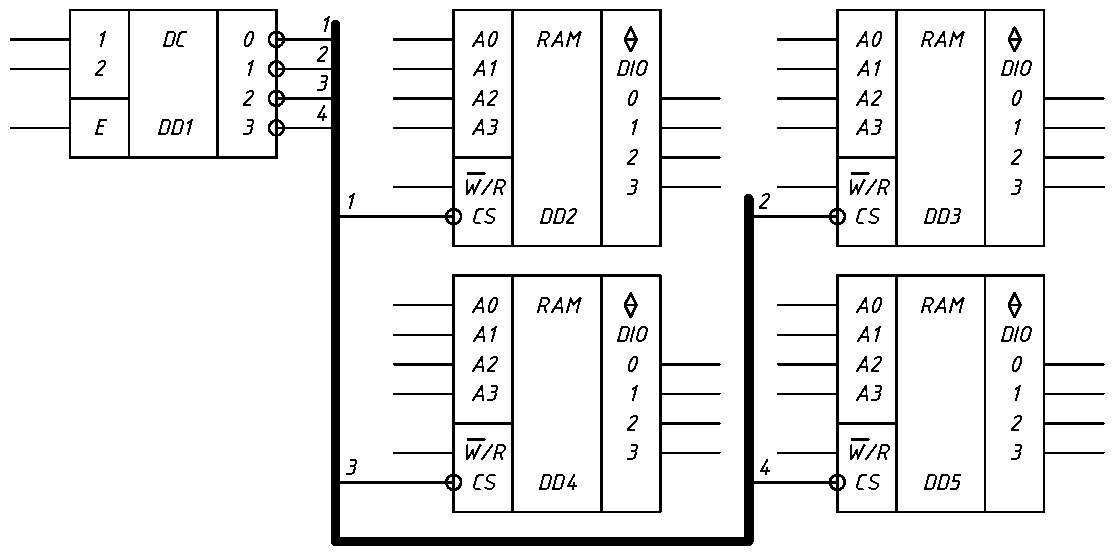
\includegraphics[width=\textwidth]{img/shina-crop.pdf}
\caption{Оформлення лінії групового зв'язку (шини)}
\label{fig:shina}
\end{figure}

Для однозначного визначення елементів, що входять до складу виробу і зображених на схемі, кожному елементу або пристрою схеми присвоюють літерно-цифрове позиційне позначення згідно з ГОСТ 2.710-81.

	Позиційне позначення в загальному випадку складається з трьох частин. У першій частині вказують вид елемента (пристрою) однією або декількома літерами, наприклад, {\gostfnt R} — резистор, {\gostfnt С} — конденсатор (для уточнення виду елемента допускається застосовувати двох літерний код, наприклад, для цифрової мікросхеми — {\gostfnt DD}); у другій частині — порядковий номер елемента або пристрою в межах даного виду, наприклад: {\gostfnt R1, R2, ..., R6}\textit{;} {\gostfnt С1, С2, ..., С5}\textit{;} {\gostfnt DD1, DD2}\textit{;} у третій частині допускається вказувати відповідне функціональне призначення, наприклад {\gostfnt C2I} -- конденсатор {\gostfnt С2}, що використовується як інтегрувальний. 

Позиційні позначення елементам (пристроям) присвоюють починаючи з одиниці в межах групи елементів (пристроїв) з однаковими позиційними позначеннями, за послідовністю розташування елементів на схемі, рахуючись згори вниз, зліва направо. Цифри порядкових номерів і їх літерні позиційні позначення виконують одним розміром шрифту.

Дані про елементи, що входять до складу виробу і зображені на схемі, записують в перелік елементів, який поміщають на першому аркуші схеми або виконують у вигляді самостійного документа певного формату (рис. \ref{fig:perelik}). 

\begin{figure}[h]
%\noindent
\centering
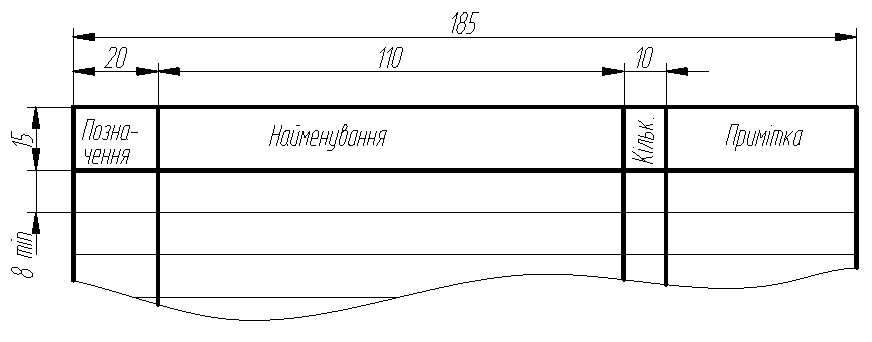
\includegraphics[width=\textwidth]{img/perelik-crop.pdf}
\caption{Оформлення переліку елементів}
\label{fig:perelik}
\end{figure}

У першому випадку перелік оформляється у вигляді таблиці, що заповнюється зверху вниз. Її розташовують, як правило, над основним написом на відстані не менше 12 мм від неї. Продовження переліку поміщають зліва від основного напису, повторюючи головку таблиці. У другому випадку перелік елементів виконується на
форматі А4 з основним написом згідно з ГОСТ 2.104–68 (форма 2 і 2а), з присвоєнням шифру, що складається з літери П (перелік) і коду схеми, до якої випускається перелік, наприклад: ПЕ3 — (П) перелік елементів до (Е) електричної (3) принципової схеми. У графах переліку елементів указують такі дані:

\begin{itemize}
\item у стовпці «Поз. позначення» наводяться позиційні позначення елементів (пристроїв);
\item у стовпці «Найменування» — найменування елементів (пристроїв) відповідно до документа, на підставі якого цей елемент (пристрій) застосований, а також позначення цього документа (основний конструкторський документ: ГОСТ, ТУ);
\item у стовпці «Кількість» — кількість однакових елементів;
\item у стовпці «Примітка» — технічні дані елемента, що не містяться в його найменуванні (за необхідності).
\end{itemize}

Допускається всі відомості про елементи поміщати поряд з їх зображенням на вільному полі схеми. Зв’язок переліку елементів має здійснюватися через позиційні позначення.

Перелік заповнюється згори вниз як у випадку, коли перелік розташований на першому аркуші схеми, так і у разі виконання його у вигляді самостійного документа (рис. \ref{fig:elist}). Заповнення переліку проводять групами в алфавітному порядку літерно-цифрових позиційних позначень. Якщо на схемі застосовуються позиційні позначення з літер латинського і українського алфавітів, то в перелік спочатку записують елементи з позиційними позначеннями з літер латинського алфавіту, а потім -- українського. В межах кожної групи, що має однакові літерні позиційні позначення, елементи розташовуються за збільшенням порядкових номерів. Між окремими групами елементів рекомендується залишати декілька незаповнених рядків для внесення змін.

\begin{figure}[h]
%\noindent
\centering
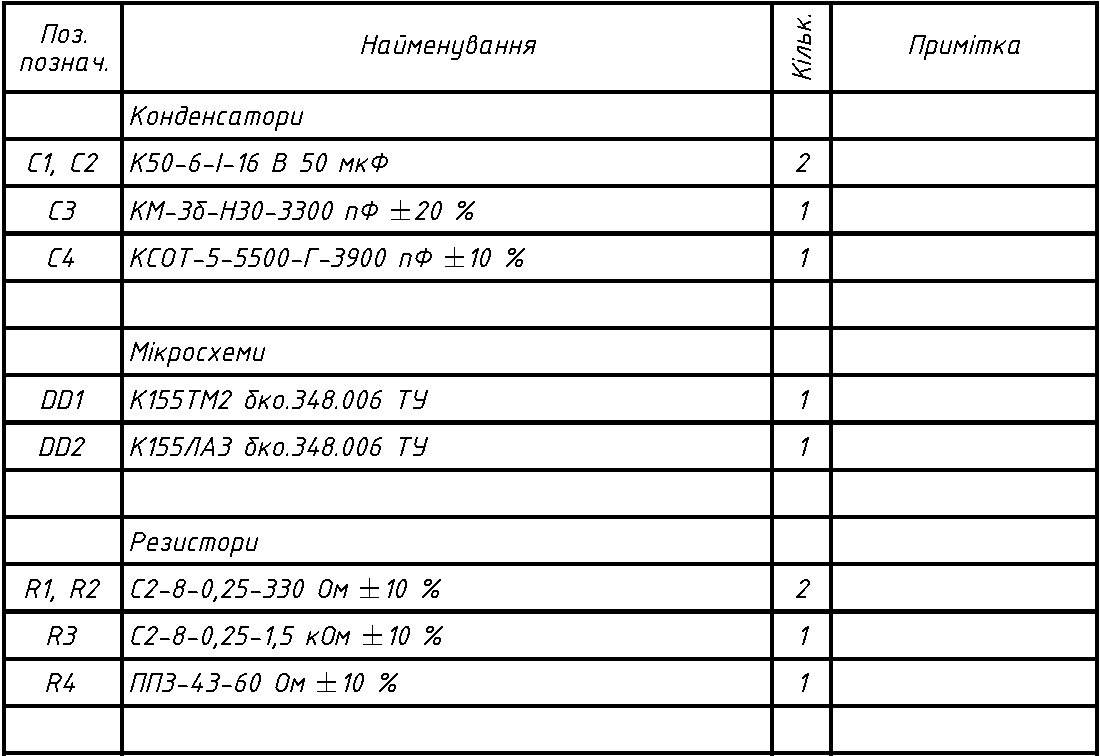
\includegraphics[width=0.9\textwidth]{img/elist-example.pdf}
\caption{Приклад заповнення переліку елементів}
\label{fig:elist}
\end{figure}
 